\chapter{ComStock Workflow}

Accurately representing commercial building energy usage is complex because of how subsystems of a building interact with one another and with the surrounding environment. Every aspect of a commercial building can influence its energy consumption, so it is difficult to identify which aspects of a building are critical for a given energy-related metric and climate without simulation. To achieve its fundamental goal of representing the U.S. commercial building stock across all energy-related metrics, ComStock must capture the diversity and variability of the building stock. This requires a robust modeling and publishing workflow. 

At the heart of ComStock are the approximately 350,000 building energy models (BEMs) that collectively represent the commercial building stock in the United States (roughly 6 million buildings). These models do not represent specific individual buildings (for example, there is no ComStock model for the Empire State Building). Modeling individual buildings would be impractical given the difficulty of compiling accurate data on the U.S. building stock at a national scale. Identifying distributions of characteristics is a more tractable problem. For example, the EIA's Commercial Buildings Energy Consumption Survey (CBECS) \citep{eia2012cbecs} provides information on how many buildings by type have specific heating, ventilating, and air-conditioning (HVAC) system characteristics (e.g., an office building with a chiller). Combining this information with a building's size and when and where it was built has allowed the ComStock team to develop statistical distributions that determine the characteristics for each of the 350,000 models.

Creating and running the 350,000 BEMs that lie at the heart of ComStock---and then sharing the results---requires significant infrastructure. The workflow that defines, executes, and post-processes these BEMs is shown in Figure \ref{fig:comstock_workflow}. The remainder of this section contains an abridged discussion of the elements of this workflow and their role in creating the ComStock BEMs and the results data set. Each aspect of the workflow is revisited in detail in Section 4 as modeling assumptions and algorithms are discussed.

\begin{figure}[h!]
  \centering
  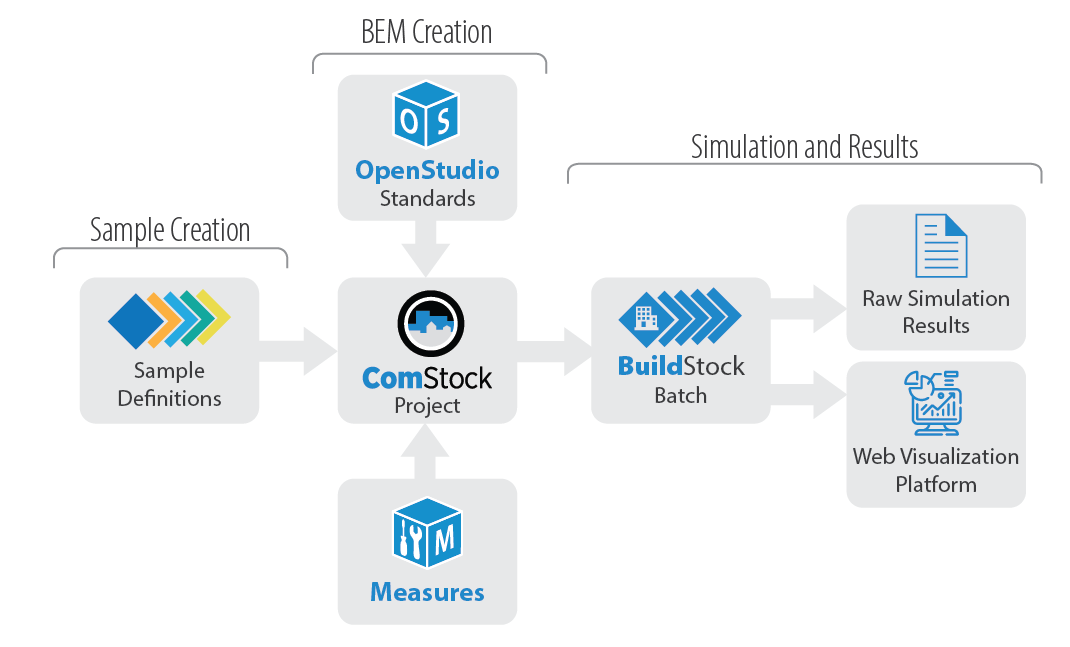
\includegraphics[width=\textwidth]{figures/comstock_workflow.png}
  \caption[Flowchart of the ComStock workflow]{Flowchart of the ComStock workflow.}
  \label{fig:comstock_workflow}
\end{figure}

\pagebreak

ComStock accomplishes its goal of accurately representing the U.S. building stock through a three-part workflow process: \begin{enumerate}
    \item ComStock creates samples that represent the U.S. commercial building stock.
    \item These samples are translated into BEMs and modified to represent either the baseline U.S. commercial building stock or an altered version thereof (i.e., modeling the impact of an efficiency or electrification measure).
    \item The physics-based BEMs are evaluated through an energy simulation engine that uses high-performance computing to simulate each model. The resulting data are made available to a wide range of stakeholders.
\end{enumerate}

\section{ComStock Sample Definitions}
\label{sec:sample_definitions}

ComStock uses a number of publicly and privately available databases that define what buildings exist, where they are located, when they were built, and with what characteristics they have. The characteristics include (but are not limited to) floor area, HVAC system type, and window type, as well as building-type-specific characteristics such as number of beds (for hospitals) or number of students (for educational institutions). When assembled, these data sets provide the basis for representing the U.S. commercial building stock.

The input data sets used to develop ComStock are often the result of extensive, highly capital-intensive data collection efforts. Some of the data sets purchased for this work are subject to data retention clauses that require deletion of the raw data after the contractual use has been completed. Given these contractual agreements, ComStock typically aggregates and joins with other data sets to generate distributional estimates of relationships between key characteristics. These input distributions are the first step in generating samples for ComStock.

Translating the input distributions into individual samples, or combinations of characteristics, requires a sampling process. Currently, ComStock assembles all input distributions as an $n$-dimensional joint probability distribution, which is then sampled using a space-filling sampling algorithm. The goal of the sampling algorithm is to minimize the largest void, or ``gap,'' between individual samples.

Each sample generated by the sampling algorithm defines the input characteristics for a single BEM. This results in hundreds of thousands of BEMs (millions when alterations to the building stock are also considered). Each of these BEMs must be created through automated model-generation scripts (discussed in Section~\ref{sec:openstudio_standards}) and evaluated via a BEM physics engine (discussed in Section~\ref{sec:buildstockbatch}). Additionally, it is often necessary to consider the impact of alterations or retrofits to the building stock---the development and use of Measures are discussed in the following section (Section~\ref{sec:measures}).

\section{Measures for ComStock}
\label{sec:measures}

A major advantage of physics-based models is their ability to change the inputs and evaluate the effect on the outputs. For ComStock, such changes are primarily evaluated using Energy Efficiency Measures or Electrification Measures. Although the word \emph{measure} has a generally accepted meaning in the energy efficiency industry, when capitalized henceforth, \emph{Measure} indicates a script that can be executed on the ComStock BEMs to alter the model inputs. A collection of Measures is a collection of scripts that allow various alterations---such as energy efficiency interventions, electrification interventions, or demand-response strategies/technologies---to be applied across the 350,000 BEMs that comprise a national run with ComStock. These automated alterations are a key aspect of ComStock's value proposition.

Throughout ComStock's development, various Measures have been developed for specific projects. These include Measures developed to support the Los Angeles 100\% Renewable Energy Study (LA100), the Advanced Building Construction Typology Report, and, in ComStock's infancy, the Electrification Futures Study. Currently, the ComStock team is developing a more robust and generalized set of Measures that will be published. These Measures are still in development, but at minimum will include efficiency and electrification Measures.

A key element of Measures is the interconnected nature of the intervention and the BEM representation of building systems and technologies. As an example, when modeling an intervention that adds an economizer to all rooftop units without an economizer, the modeling workflow relies on (a) the Measure identifying which rooftop units already have an economizer, and (b) the Measure updating the BEMs that do not have an economizer.

In the case of a Measure that electrifies forklifts in warehouses, however, two issues arise. First, none of ComStock's sample definition characteristics provide information on which warehouses (or other building types) this measure is applicable to, or to what degree. Second, there is no disambiguation of forklift load vs. other internal load in ComStock. As such, any Measure that attempts to implement this intervention has to rely on scaled measurement and verification or market research studies. In both cases, the estimates may be accurate, but it is difficult to tie the impact to any fundamental characteristic of the model and represent the variability of the impact across buildings. Although this does not invalidate the value of such a measure, it is important to differentiate measures that fit into ComStock's sample definitions and OpenStudio-Standards' workflow from those that are ``bolted on'' post-hoc.

\section{OpenStudio-Standards}
\label{sec:openstudio_standards}

OpenStudio-Standards is an open-source modeling library that defines the detailed inputs of a BEM based on simple input values. It contains the software needed to add all building systems for each vintage of every building type. This software is primarily based on the building energy code at the time of construction/retrofit. It contains the software code needed to add all building systems for each vintage of every building type, primarily based on building energy code followed by the building at time of construction/retrofit. This capability is paired with a set of space types that represent the loads of a specific building type to allow for complete model definition.

OpenStudio-Standards was originally developed to help automate the process of creating energy code baseline BEMs. This allowed for more consistent creation of baseline models for efficiency incentive programs. Throughout the development and calibration of ComStock, these code-minimum assumptions have been altered to better reflect the building performance seen in measured data sources. In some cases, this has resulted in components being defined on a non-code basis (e.g., LEDs), whereas in other cases, calibration has resulted in alterations to the nominal assumptions in code-minimum definitions. These alterations are discussed in detail in the relevant subsections of Section~\ref{chap:4_modeling}.

OpenStudio-Standards was not originally developed for ComStock and is used for many other purposes. The standards represent the collaborative work of many researchers at Lawrence Berkeley National Laboratory, Pacific Northwest National Laboratory, and Oak Ridge National Laboratory.

\section{ComStock Project}

A ComStock project includes a baseline building stock definition and a selection of Measures. For example, a ComStock project that analyzes the building envelope savings potential for the state of Colorado would include all building samples in Colorado and Measures that capture several efficiency levels for walls, roofs, and windows. The results of this project would identify the energy impacts of bringing Colorado commercial building envelopes up to code and/or above code.

Results for a ComStock project are relative to a fixed point in the lifespan of the building stock. For example, ComStock currently represents the building stock as it looked in 2018. Results assume overnight adoption of changes to the building stock. In reality, large-scale changes to the building stock take many years, and the building stock evolves during that process. If either the baseline building stock characteristics or the measures being considered change significantly, careful consideration of the applicability of results is needed. In many cases, the changes in the point in time and the measures being considered will not significantly change the results. However, in some cases, a rapidly evolving understanding of technology performance and saturation, or increasingly refined questions, will trigger the need for updated or refined analyses. For example, state-of-the-art air-source heat pump characteristics may change rapidly, making results from a ComStock project using older technology assumptions obsolete.

\section{BuildStockBatch}
\label{sec:buildstockbatch}

BuildStockBatch is a software library that executes ComStock and ResStock projects. ResStock is a residential building sector model and shares many workflow components with ComStock.  BuildStockBatch is typically used by NREL researchers on NREL's high-performance computing system, Eagle. However, the ResStock team has developed and demonstrated an Amazon Web Services (AWS)-based workflow that can be used by entities without access to the U.S. Department of Energy's (DOE's) high-performance computing system. BuildStockBatch can run up to tens of millions of simulations for a given ComStock (or ResStock) project. Although the number of simulations in these projects can vary greatly, BuildStockBatch scales by distributing simulations across a number of servers. The number of servers increases in proportion to the number of simulations, ranging from a few servers to hundreds of servers. After each server completes its requested simulations, it pushes the results to a remote file-system-based database.

Currently, BuildStockBatch utilizes an Eagle high-performance computing workflow for ComStock. In the future, ComStock expects to provide a proof-of-concept BuildStockBatch implementation that uses AWS to execute a ComStock simulation. It is not yet clear whether funding will be allocated to support this workflow's use by third-party users, but the AWS-enabled code base will be publicly available when developed.

\section{Raw Simulation Results}
\label{rawsimulationresults}
The simulation results from national ComStock releases are transferred to an AWS bucket provided by the Open Energy Data Initiative (OEDI) Data Lake partnership with AWS. This bucket contains several versions of the raw results. It contains the OpenStudio BEMs (.osm files) used to represent each sampled building. It also provides each building sample's simulated energy consumption results on a 15-minute basis, per end use, per Measure upgrade. These files are stored such that they can be queried using AWS's Athena service. Finally, the annualized results are provided on a baseline/upgrade basis, where each Measure upgrade defined in the ComStock project has its own annualized result file.

\section{Web-Based Visualization Platform}
\label{dataviewer}
ComStock and ResStock utilize a shared platform for data visualization. In most cases, users are looking for the sum or average load profile of all buildings of a given type in a given geographic area. These are referred to as ``aggregate'' load profiles. The visualization platform, which can be found at \href{comstock.nrel.gov}{comstock.nrel.gov}, provides users with an interface to interact with both annualized and 15-minute-interval data segmented by geography and building characteristic. As previously discussed, ComStock does not providet results that represent specific buildings, but rather aims to represent the distribution and variability of the building stock across the United States. Users who interact with \href{comstock.nrel.gov}{comstock.nrel.gov} generally have a more consistent and beneficial experience than those who interact with individual sample results. The results are available for several weather years and several different geographic resolutions. It is important to note that, at present, the more refined the geographic resolution, the less confidence should be placed in the results. This is because fewer samples will have been generated to approximate the relevant stock.